\documentclass{article}

\usepackage{fancyhdr} % Required for custom headers
\usepackage{lastpage} % Required to determine the last page for the footer
\usepackage{extramarks} % Required for headers and footers
\usepackage{graphicx} % Required to insert images
\usepackage{lipsum} % Used for inserting dummy 'Lorem ipsum' text into the template


% Margins
\topmargin=-0.35in
\evensidemargin=0in
\oddsidemargin=0in
\textwidth=6.5in
\textheight=9.0in
\headsep=0.25in 

\linespread{1.1} % Line spacing

% Set up the header and footer
\pagestyle{fancy}% Top left header
\rhead{} % Top right header
\lfoot{\lastxmark} % Bottom left footer
\cfoot{} % Bottom center footer
\rfoot{P\'{a}gina\ \thepage\ de\ \pageref{LastPage}} % Bottom right footer
\renewcommand\headrulewidth{0.4pt} % Size of the header rule
\renewcommand\footrulewidth{0.4pt} % Size of the footer rule

\setlength\parindent{0pt} % Removes all indentation from paragraphs

%----------------------------------------------------------------------------------------
%	DOCUMENT STRUCTURE COMMANDS
%	Skip this unless you know what you're doing
%----------------------------------------------------------------------------------------



\setcounter{secnumdepth}{0} % Removes default section numbers
\newcounter{homeworkProblemCounter} % Creates a counter to keep track of the number of problems

\newcommand{\homeworkProblemName}{}
\newenvironment{homeworkProblem}[1][Parte \arabic{homeworkProblemCounter}]{ % Makes a new environment called homeworkProblem which takes 1 argument (custom name) but the default is "Problem #"
\stepcounter{homeworkProblemCounter} % Increase counter for number of problems
\renewcommand{\homeworkProblemName}{#1} % Assign \homeworkProblemName the name of the problem
\section{\homeworkProblemName} % Make a section in the document with the custom problem count

}

\newcommand{\problemAnswer}[1]{ % Defines the problem answer command with the content as the only argument
\noindent\framebox[\columnwidth][c]{\begin{minipage}{0.98\columnwidth}#1\end{minipage}} % Makes the box around the problem answer and puts the content inside
}

\newcommand{\homeworkSectionName}{}
\newenvironment{homeworkSection}[1][Parte \arabic{homeworkProblemCounter}]{ % New environment for sections within homework problems, takes 1 argument - the name of the section
\renewcommand{\homeworkSectionName}{#1} % Assign \homeworkSectionName to the name of the section from the environment argument
\subsection{\homeworkSectionName} % Make a subsection with the custom name of the subsection
}{
}
   
%----------------------------------------------------------------------------------------
%	NAME AND CLASS SECTION
%----------------------------------------------------------------------------------------

\newcommand{\hmwkTitle}{Empresa XXX S.A.} % Assignment title
\newcommand{\hmwkDueDate}{Mi\'{e}rcoles,\ Mayo\ 25,\ 2016} % Due date
\newcommand{\hmwkClass}{GC} % Course/class
\newcommand{\hmwkClassInstructor}{Maria Jose Gils} % Teacher/lecturer
\newcommand{\hmwkAuthorName}{Gorka Barturen y Carlos Perales} % Your name

%----------------------------------------------------------------------------------------
%	TITLE PAGE
%----------------------------------------------------------------------------------------

\title{
\vspace{2in}
\textmd{\textbf{\hmwkClass:\ \hmwkTitle}}\\
\normalsize\vspace{0.1in}\small{\hmwkDueDate}\\
\vspace{3in}
}

\author{\textbf{\hmwkAuthorName}}
\date{} % Insert date here if you want it to appear below your name

%----------------------------------------------------------------------------------------

\begin{document}

\maketitle

%----------------------------------------------------------------------------------------
%	TABLE OF CONTENTS
%----------------------------------------------------------------------------------------

%\setcounter{tocdepth}{1} % Uncomment this line if you don't want subsections listed in the ToC

\newpage
\tableofcontents
\newpage

%----------------------------------------------------------------------------------------
%	PROBLEM 1
%----------------------------------------------------------------------------------------

% To have just one problem per page, simply put a \clearpage after each problem

\begin{homeworkProblem}[1.1. Visi\'{o}n, Misi\'{o}n y estrategia]
Visi\'{o}n:
\begin{itemize}

\item Ser la empresa l\'{i}der en Espa\~{n}a en la venta de electrodom\'{e}sticos.
\item Ser una empresa que trabaje tanto por la sostenibilidad de s\'{i} misma como por la de sus productos.
\item Ampliar la infraestructura de la empresa a nivel internacional.
\item Mejora del ciclo de vida de los productos.

\end{itemize}

Misi\'{o}n: Ser la empresa que produce los electrodom\'{e}sticos sostenibles con mejor relaci\'{o}n calidad-precio.

\end{homeworkProblem}
\clearpage

%----------------------------------------------------------------------------------------
%	PROBLEM 2
%----------------------------------------------------------------------------------------
\begin{homeworkProblem}[1.2. Identificaci\'{o}n de los conocimientos pertinentes ]

\begin{homeworkSection}[a. Auditor\'{i}a del conocimiento inicial]  % Custom section title
Auditor\'{i}a de sistemas:
\begin{itemize}

\item SAP  (Sistema ERP)
\item Oracle (SGBD)
\item Procesadores de textos 
\item Intranet/Extranet
\item DSS
\item Sistemas expertos
\item Agentes inteligentes
\item Voice on IP (Skype, Teamspeak…)
\item Videoconferencias (Skype, hangouts...)
\item Messengers (Whatsapp, telegram…)
\item E-mail (Gmail, Outlook…)
\item VPN
\item Sistemas legados

\end{itemize}

Auditor\'{i}a de personas:

\begin{itemize}

\item Accionistas de la asamblea general
\item Miembros de la asamblea permanente
\item Director general
\item Representantes de cada departamento

\end{itemize}


\end{homeworkSection}
\clearpage

%----------------------------------------------------------------------------------------
%	PROBLEM 3
%----------------------------------------------------------------------------------------

\begin{homeworkSection}[b. An\'{a}lisis DAFO] % 
Debilidades:
\begin{itemize}

\item A pesar de ser reconocidos en Espa\~{n}a, no tenemos demasiado mercado fuera del pa\'{i}s
\item Alto coste de fabricaci\'{o}n para mantener nuestra calidad

\end{itemize}

Amenazas:

\begin{itemize}

\item Que otras empresas compitan contra nosotros centr\'{a}ndose en nuestra ventaja competitiva y bajen los costes del producto
\item Que no consigamos expandirnos fuera de Espa\~{n}a por alg\'{u}n problema de legislaci\'{o}n.

\end{itemize}

Fortalezas:

\begin{itemize}

\item Somos una marca referente en Espa\~{n}a
\item Diferentes gamas de productos para satisfacer a diferentes consumidores

\end{itemize}

Oportunidades:

\begin{itemize}

\item Nuevos mercados con necesidades b\'{a}sicas que cubrimos gracias a nuestra amplia gama de productos

\end{itemize}


Iniciativas de Gesti\'{o}n de Conocimiento
\begin{itemize}

\item Hacer las p\'{a}ginas amarillas con el conocimiento de cada empleado, estableciendo as\'{i} un documento que recoge todos los perfiles de conocimiento de la empresa para futuras formaciones de grupos y b\'{u}squeda de requisitos en la empresa.

\item Potenciar el mercado internacional aprovechando los mercados emergentes y nuestra amplia gama de productos. 
\begin{enumerate}

\item Analizar los perfiles de los empleados para escoger a los componentes de un equipo que se centrar\'{a} en el an\'{a}lisis de los diferentes mercados y en valorar los riesgos y los beneficios a la hora de expandirse a un nuevo mercado.

\item Establecer un equipo de adaptaci\'{o}n de mercado, que establezca un plan para poder adaptar nuestra empresa a las necesidades del nuevo mercado a la hora de expandirnos. 
Este equipo se encargar\'{a} tambi\'{e}n de la b\'{u}squeda de debilidades en los mercados, aprovechando las oportunidades que dejan otras empresas para poder impulsarnos de forma m\'{a}s efectiva en estos nuevos mercados.

\end{enumerate}

\item Conseguir que nuestra ventaja competitiva resida en la calidad, de esta forma no habr\'{a} ning\'{u}n problema en competencia de costes. 

\begin{enumerate}
\item Analizar los perfiles de los empleados para elegir a los expertos en procesos de calidad o para establecer grupos de formaci\'{o}n en procesos de calidad.

\item Establecer un equipo de empleados que analice y monitorice nuestro proceso de calidad para poder reforzarlos, mejorando as\'{i} la calidad de nuestros productos.
\end{enumerate}
\item Llevar al d\'{i}a los permisos y legislaciones de los nuevos mercados internacionales a los que nos queramos expandir.
Analizar los perfiles de los empleados para poder crear un grupo centrado en llevar al d\'{i}a la legislaci\'{o}n vigente del mercado internacional. [  ]

\item Aprovechar nuestra fortaleza en Espa\~{n}a para empezar a expandir el mercado en pa\'{i}ses afines a este.
Analizar el proceso de expansi\'{o}n en Espa\~{n}a y capturar c\'{o}mo se ha desarrollado durante el tiempo para poder replicarlo y mejorarlo en esos pa\'{i}ses.

\item Aprovechar posibles carencias en otros mercados que conseguimos cubrir con nuestros productos, para as\'{i} impulsar a nuestra empresa de forma m\'{a}s efectiva explotando las debilidades de otras empresas.



\end{itemize}

\end{homeworkSection}
\clearpage

%------------------------------------------------------------------------

\begin{homeworkSection}[c. P\'{a}ginas amarillas] % Custom section title

\begin{itemize}


\item ¿D\'{o}nde guardaremos esta informaci\'{o}n?\\
La informaci\'{o}n de cada empleado estar\'{a} guardada en una base de datos relacional en la que se dividir\'{a}n todos estos datos en tablas, manteniendo as\'{i} un registro ordenado sobre cada una de las caracter\'{i}sticas de los empleados.
\item ¿De d\'{o}nde recogemos la informaci\'{o}n?\\
La informaci\'{o}n de los perfiles de este documento se recoger\'{a} y se actualizar\'{a} desde la base de datos del departamento de recursos humanos, por lo que los empleados no ser\'{a}n los encargados de introducir esta informaci\'{o}n.
\item ¿C\'{o}mo accederemos a ella?\\
Se podr\'{a} acceder a todas las fichas de empleados y a su informaci\'{o}n mediante un buscador, en el cual se filtrar\'{a} la b\'{u}squeda mediante diferentes m\'{e}todos (nombre, proyecto, cursos, tags de conocimiento…) y se visualizar\'{a} una lista de resultados en forma de fichas de empleados que pasen los filtros.
Tambi\'{e}n se puede acceder a informaci\'{o}n sobre cursos, departamentos, proyectos… desde los hiperv\'{i}nculos de la propia ficha del empleado desde la cual se redirigir\'{a} al usuario a la informaci\'{o}n buscada.

\begin{center}
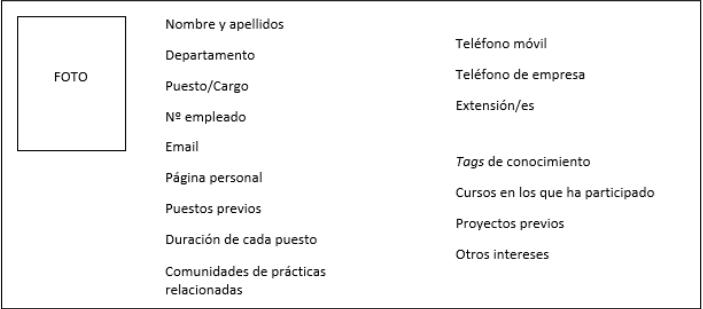
\includegraphics[width=0.85\columnwidth]{PA} % Example image
\end{center}
\end{itemize}
\end{homeworkSection}
\clearpage

%--------------------------------------------

\begin{homeworkSection}[d. Lista de procesos] 

\begin{itemize}
\item (E)An\'{a}lisis de la trayectoria a nivel nacional de la empresa (buenas pr\'{a}cticas)
\item (E)Satisfacci\'{o}n de los empleados
\item (E)An\'{a}lisis y reducci\'{o}n del impacto medioambiental del proceso de producci\'{o}n 
\\

\item (O)Atenci\'{o}n al cliente
\item (O)Mejora del proceso de fabricaci\'{o}n de electrodom\'{e}sticos
\item (O)Formaci\'{o}n / Adecuaci\'{o}n de los empleados a los puestos
\\

\item (S)Gesti\'{o}n adecuada de nuestros empleados
\item (S)Mejora en la gesti\'{o}n de los materiales
\item (S)Atenci\'{o}n a las sugerencias y reclamaciones (clientes y empleados)

\end{itemize}
\end{homeworkSection}
\clearpage

%----------------------------------------------------------------------------------------

%----------------------------------------------------------------------------------------

\begin{homeworkSection}[e. Definici\'{o}n de procesos ] % Custom section title
\begin{center}
Mejora del proceso de fabricaci\'{o}n de electrodom\'{e}sticos

\begin{itemize}

\item Objetivos:  Mejorar nuestro proceso de fabricaci\'{o}n para conseguir mejorar nuestra ventaja competitiva frente a la competencia
\item Inicio: Buscar en los perfiles de los empleados para encontrar a los m\'{a}s adecuados
\item Fin: Asignar a las personas id\'{o}neas al grupo
\item Propietario: El encargado de ese \'{a}mbito (Champion)
\item Cliente: La misma empresa es la que est\'{a} interesada en llevar a cabo el proceso
\item Proveedor: La propia empresa es la proveedora
\begin{center}

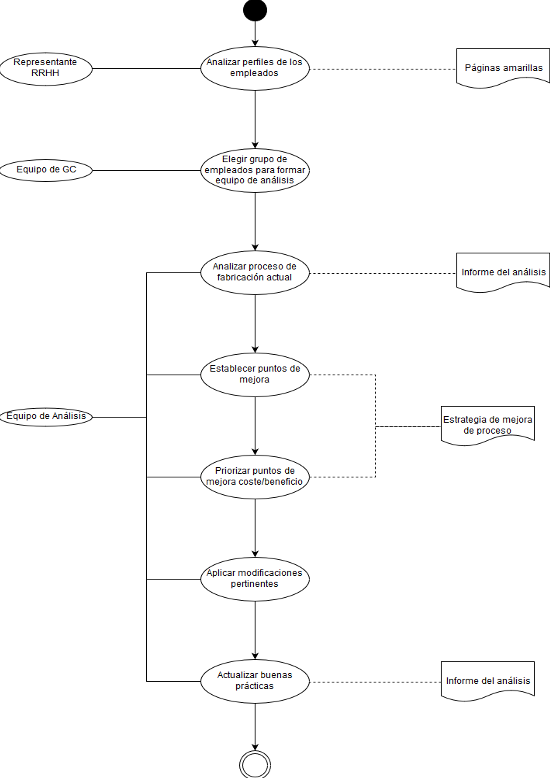
\includegraphics[height=0.75\columnwidth]{pFab} % Example image
\end{center}
\clearpage
\end{itemize}

Potenciar un marketing a nivel internacional

\begin{itemize}
\item Objetivos: Potenciar el mercado internacional aprovechando los mercados emergentes y nuestra amplia gama de productos
\item Inicio: Analizar a los empleados que van a estar encargados
\item Fin: Ser los putos amos del mundo
\item Propietario: El encargado del departamento de marketing
\item Cliente: La misma empresa es la que est\'{a} interesada en llevar a cabo el proceso
\item Proveedor: La propia empresa es la proveedora

\begin{center}

\includegraphics[width=0.75\columnwidth]{MarketInt} % Example image
\end{center}

\end{itemize}
\end{center}

\end{homeworkSection}
\clearpage

%----------------------------------------------------------------------------------------

\begin{homeworkSection}[f. Identificaci\'{o}n de los procseos] % Custom section title

Los procesos del apartado 1.2.d que est\'{a}n relacionados con nuestras iniciativas de gesti\'{o}n del conocimiento son los siguientes:
\begin{itemize}

\item Lograr un marketing efectivo a nivel internacional: este proceso est\'{a} relacionado con nuestra iniciativa de potenciaci\'{o}n del mercado a nivel internacional. Al conseguir realizar este proceso con \'{e}xito, conseguiremos aumentar la presencia internacional de nuestra empresa y por consiguiente, mejorar las ventas.

\item An\'{a}lisis y reducci\'{o}n del impacto medioambiental del proceso de producci\'{o}n: este proceso est\'{a} relacionado con nuestra iniciativa de crear un equipo de empleados que analice y monitorice nuestro proceso de calidad de la producci\'{o}n de nuestros productos. Consiguiendo realizar correctamente este proceso, conseguiremos potenciar nuestra ventaja competitiva (calidad de la producci\'{o}n).

\item Mejora del proceso de fabricaci\'{o}n de los electrodom\'{e}sticos: este proceso est\'{a} muy relacionado tanto con el proceso anterior como con la iniciativa del mismo. 

\item Formaci\'{o}n de los empleados: este proceso es uno de los procesos m\'{a}s importantes de nuestro proceso de gesti\'{o}n del conocimiento, ya que para llevar a cabo las iniciativas en las que necesitamos un equipo, el conocimiento de nuestro personal tiene que estar actualizado, por lo que la formaci\'{o}n es algo esencial.

\item Gesti\'{o}n adecuada de nuestros empleados: en la creaci\'{o}n de los grupos de gesti\'{o}n de conocimiento para diversas iniciativas, tenemos que llevar una gesti\'{o}n de nuestro personal 

\item Mejora de la gesti\'{o}n de los materiales: este proceso est\'{a} relacionado con la iniciativa de an\'{a}lisis y monitorizaci\'{o}n del proceso de calidad de la producci\'{o}n de nuestros productos, ya que el hecho de llevar una gesti\'{o}n m\'{a}s evolucionada, puede ayudar a nuestra empresa a competir en costes con la competencia.

\end{itemize}
\end{homeworkSection}
\clearpage


%----------------------------------------------------------------------------------------
\begin{homeworkSection}[h. Identificar las fuentes externas de conocimiento] % Custom section title
\begin{itemize}
\item Proveedores: Nuestras iniciativas para la mejora de la calidad de nuestros productos requieren que la calidad de los materiales que nos proporcionan nuestros proveedores sea la m\'{a}s alta posible por lo que el conocimiento de los proveedores es uno de los pilares fundamentales de nuestra estrategia de gesti\'{o}n del conocimiento.
\item Gobierno/Legislaci\'{o}n: Esta fuente nos proporciona informaci\'{o}n sobre los aspectos legales del mercado y de la producci\'{o}n aportando los cambios y modificaciones de las leyes que rigen el comportamiento de los procesos.
\item Empresas de formaci\'{o}n externas: Estas empresas aportan el conocimiento asociado a la formaci\'{o}n, es decir, estas empresas aportan se dedican a formar y con esta actividad aparece trasladan su conocimiento a nuestros empleados, lo que conlleva tambi\'{e}n traslado de conocimiento a nuestra empresa.
\end{itemize}

\end{homeworkSection}
\end{homeworkProblem}
\clearpage


%----------------------------------------------------------------------------------------
\begin{homeworkProblem}[1.3. Estudio de viabilidad] % Custom section title
\begin{itemize}
\item Viabilidad econ\'{o}mica: nuestras iniciativas tienen un coste considerablemente bajo comparado con los beneficios que pueden llegar a aportar. Esto se debe a que para la gran mayor\'{i}a de ellas, vamos a utilizar a nuestra propia fuerza de trabajo por lo que los costes de contrataci\'{o}n/ampliaci\'{o}n de contratos, van a ser bajos. Para las iniciativas de mejora de nuestros propios trabajadores utilizaremos empresas externas que pueden subir el coste de la iniciativa pero los beneficios que esperamos de las iniciativas superan ampliamente a los costes.

\item Viabilidad t\'{e}cnica: todas las necesidades tecnol\'{o}gicas relacionadas con nuestras iniciativas las tenemos ya en nuestra empresa menos las necesarias para el desarrollo de las p\'{a}ginas amarillas. Para la mejora del proceso de calidad puede ser que necesitemos m\'{a}s herramientas pero no consideramos que estos costes vayan a ser demasiado elevados.
 
\item Viabilidad del proyecto: en nuestra opini\'{o}n todas nuestras iniciativas son realistas y se pueden llevar a cabo en el tiempo adecuado para el correcto desarrollo del proceso de gesti\'{o}n del conocimiento.

\end{itemize}

\end{homeworkProblem}

%----------------------------------------------------------------------------------------
\begin{homeworkProblem}[1.4. Definici\'{o}n de Indicadores de Gesti\'{o}n del Conocimiento] % Custom section title

\begin{itemize}
\item La Actividad: nivel de uso y aprovechamiento de los distintos procesos y canales de gesti\'{o}n del conocimiento-> 
Nº de usuarios, Nº de miembros, Nº de consultas...
\end{itemize}

\begin{itemize}
\item El Conocimiento: nivel de conocimiento generado y/o registrado y su nivel de consumo o aprovechamiento-> 
Nº de buenas pr\'{a}cticas generadas, Nº de lecciones aprendidas generadas, Nº de ideas propuestas...
\end{itemize}

\begin{itemize}
\item Los Impactos o beneficios que se est\'{a}n obteniendo, tanto cualitativos como cuantitativos-> 
Nº de personas que han mejorado su formaci\'{o}n, nº de miembros en proyectos de mejora de la calidad, Nº de casos que se resuelven con el conocimiento existente...
\end{itemize}

Mejora del proceso de calidad de electrodom\'{e}sticos

\begin{itemize}
\item El Conocimiento: nivel de conocimiento generado y registrado y su nivel de consumo o aprovechamiento para la mejora del proceso de calidad:
\begin{itemize}
\item Nº de de buenas pr\'{a}cticas creadas y el nivel de utilizaci\'{o}n de las mismas (>10/a\~{n}o)
\item Nº de lecciones aprendidas creadas a partir de las buenas pr\'{a}cticas y el nivel de utilizaci\'{o}n de las mismas (>10/a\~{n}o)
\item Nº de ideas propuestas para la mejora del proceso de calidad (>50/a\~{n}o)
\end{itemize}
\item La Actividad: nivel de uso y aprovechamiento de los distintos procesos y canales de gesti\'{o}n del conocimiento:
\begin{itemize}
\item Nº de usuarios que utilizan el conocimiento generado (>100/d\'{i}as)
\item Nº de miembros que adem\'{a}s de utilizar el conocimiento, lo actualizan y mejoran (>10/d\'{i}as)
\item Nº de consultas que se realizan a la base de datos creada (>500/d\'{i}as)
\end{itemize}
Las m\'{e}tricas que se utilizar\'{a}n para medir si esta iniciativa est\'{a} teniendo \'{e}xito son las que est\'{a}n entre par\'{e}ntesis en los indicadores previamente descritos.
\end{itemize}


Potenciar un marketing a nivel internacional

\begin{itemize}
\item El Conocimiento: nivel de conocimiento generado y su utilizaci\'{o}n para la mejora del marketing en el extranjero
\begin{itemize}
\item Nº de de buenas pr\'{a}cticas creadas y el grado de adecuaci\'{o}n tanto para un mercado en concreto como en general
\item Nº de lecciones aprendidas creadas a partir de las buenas pr\'{a}cticas
\item Nº de ideas propuestas para la expansi\'{o}n de la empresa en el extranjero
\end{itemize}
\item La Actividad: nivel de uso y aprovechamiento de los distintos procesos y canales de gesti\'{o}n del conocimiento
\begin{itemize}
\item Nº de usuarios que utilizan el conocimiento generado
\item Nº de miembros que adem\'{a}s de utilizar el conocimiento lo aplican de manera innovadora en diferentes tipos de mercados
\item Nº de consultas que se realizan a la base de datos creada, el nivel de aprovechamiento de la misma y la expansi\'{o}n del conocimiento
\end{itemize}
\end{itemize}







\end{homeworkProblem}
\clearpage

%----------------------------------------------------------------------------------------
\begin{homeworkProblem}[2.1. Definir el ciclo de vida de GC propuesto por esta iniciativa y establecer reglas y horarios] 
El ciclo de vida del sistema de gesti\'{o}n del conocimiento propuesto comienza con la captura del conocimiento y su almacenamiento en las p\'{a}ginas amarillas. Comenzando con esta actividad conseguimos que el resto de las iniciativas sean m\'{a}s eficaces ya que los equipos encargados de llevarlas a cabo ser\'{a}n creados m\'{a}s f\'{a}cilmente y de una manera m\'{a}s \'{o}ptima. \\ \\
En segunda instancia, para las diferentes iniciativas, se crear\'{a} el equipo de gesti\'{o}n del conocimiento y este equipo se encargar\'{a} de realizar la iniciativa en concreto. \\ \\
Una vez se termine la iniciativa (la cual utilizar\'{a} el conocimiento existente en el momento actual en la empresa), se actualizar\'{a} el conocimiento introduciendo las buenas pr\'{a}cticas y las lecciones aprendidas en la realizaci\'{o}n de la misma.\\ \\
\end{homeworkProblem}

%----------------------------------------------------------------------------------------
\begin{homeworkProblem}[2.2. Definici\'{o}n de plataformas t\'{e}cnicas, el sistema de gesti\'{o}n de documentos, herramientas y t\'{e}cnicas] % Custom section title
\begin{itemize}
\item Comunidad de pr\'{a}cticas: implementaremos esto como un foro en el que cualquier empleado podr\'{a} preguntar cualquier duda que le pueda surgir a la hora de implementar una soluci\'{o}n a un problema o cualquier sugerencia que se le ocurra y el resto de los empleados podr\'{a}n aconsejarle/ plantearle soluciones para su problema y/o indicar si ese problema ha surgido en el pasado. Eventualmente, los threads m\'{a}s utilizados y m\'{a}s \'{u}tiles, pasar\'{a}n a la secci\'{o}n de buenas pr\'{a}cticas.

\item Buenas pr\'{a}cticas: una vez una soluci\'{o}n sea utilizada de manera consistente y sea aprobada por los expertos en el \'{a}mbito (una soluci\'{o}n a un problema concreto que se da numerosas veces) pasar\'{a} a ser considerado una buena pr\'{a}ctica y pasar\'{a} a esta secci\'{o}n de la plataforma implementada previamente.

\item Lecciones aprendidas: cuando una buena pr\'{a}ctica sea consistentemente utilizada y mejorada, pasar\'{a} a formar parte de las lecciones aprendidas de la empresa. En este apartado se detallar\'{a} tanto el problema, como todas las implementaciones de soluciones que se hayan dado a lo largo del tiempo (en el estilo de un log de soluciones posibles desarrolladas a lo largo de la historia de la empresa) con la \'{u}ltima soluci\'{o}n (en teor\'{i}a deber\'{i}a ser la m\'{a}s \'{o}ptima) como la recomendada para la implementaci\'{o}n.

\item P\'{a}ginas amarillas: esta parte de las iniciativas estar\'{a} relacionada en algunas partes con las comunidades de pr\'{a}cticas/ buenas pr\'{a}cticas/ lecciones aprendidas pero a\~{n}adir\'{a} mucha m\'{a}s informaci\'{o}n de los empleados como su formaci\'{o}n, los cursos en los que han participado… (como se menciona en un apartado previo).

\end{itemize}
\end{homeworkProblem}
\clearpage

%----------------------------------------------------------------------------------------
\begin{homeworkProblem}[3.1. Identificaci\'{o}n del equipo GC] % Custom section title
\begin{itemize}

\item Champion: persona encargada de promover e impulsar la gesti\'{o}n del conocimiento dentro de la empresa. Es el pilar del equipo por lo que tiene que estar completamente inmerso en el proceso de gesti\'{o}n del conocimiento.
\item Representantes de las TICs: los encargados de las TIC de la empresa (tanto de las existentes como de cualquiera de las herramientas que necesitemos para el desarrollo de nuestras iniciativas)
\item Representantes de las \'{a}reas funcionales que van involucradas en las iniciativas de gesti\'{o}n del conocimiento.

\end{itemize}

\end{homeworkProblem}

%----------------------------------------------------------------------------------------
\begin{homeworkProblem}[3.2. Estrategias para la captura del conocimiento] % Custom section title
Las estrategias de captura del conocimiento que hemos elegido utilizar est\'{a}n alineadas con nuestras iniciativas, ya que para llevar a cabo muchas de ellas, hace falta que sigamos estas directrices:
\begin{itemize}
\item Captura del conocimiento t\'{a}cito de nuestros empleados, llevaremos a cabo la captura del conocimiento usando diferentes herramientas. Para esta estrategia, las herramientas que utilizaremos ser\'{a}n evernote, entrevistas a nuestro personal, las comunidades de pr\'{a}cticas (ser\'{a}n utilizadas tanto para capturar el conocimiento como para gestionarlo y ampliarlo).
\item An\'{a}lisis del funcionamiento de los procesos de nuestra empresa y los posibles puntos en los que se puedan mejorar / debilidades de nuestros procesos.
\item Digitalizaci\'{o}n de todo el conocimiento expl\'{i}\'{i}cito que no est\'{e} computerizado para facilitar el acceso al mismo y hacer m\'{a}s sencillo el proceso de la espiral del conocimiento. Para llevar a cabo esta estrategia tambi\'{e}n se utilizar\'{a}n las comunidades de pr\'{a}cticas para que los expertos en el tema puedan a\~{n}adir al sistema los documentos que consideren relevantes y puedan descartar (o a\~{n}adir en otro apartado) los elementos que no est\'{e}n actualizados o no sean relevantes/consistentes con el estado actual de la empresa.
\end{itemize}

\end{homeworkProblem}

%----------------------------------------------------------------------------------------
\begin{homeworkProblem}[3.3. Dise\~{n}o detallado de la estructura de los documentos de cada uno de los elementos del conocimiento] % Custom section title
Los documentos que necesitaremos para el desempe\~{n}o de nuestras iniciativas son los siguientes:
\begin{itemize}
\item Buenas pr\'{a}cticas
\item Proceso + buena realizaci\'{o}n
\item Lecciones aprendidas
\item Formularios para rellenar
\item Formularios de entrevistas
\item Tests
\item Documento de alcance y viabilidad
\item P\'{a}ginas amarillas
\item P\'{a}ginas blancas
\end{itemize}
El dise\~{n}o general del encabezado de todos los documentos ser\'{a} el siguiente:
\\
\\
\begin{center}
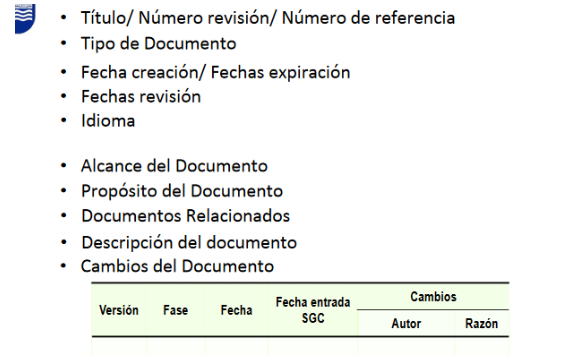
\includegraphics[width=0.75\columnwidth]{docu} % Example image
\end{center}
\clearpage

\end{homeworkProblem}
%----------------------------------------------------------------------------------------
\begin{homeworkProblem}[4.1. Formaci\'{o}n para la implementaci\'{o}n del sistema] % Custom section title

Es posible que los empleados no est\'{e}n familiarizados con las herramientas y estrategias que usaremos. 
Se organizar\'{a}n unas sesiones de formaci\'{o}n en las que se ense\~{n}\~{n}ar\'{a} a los empleados a implantar/utilizar este nuevo sistema; bien organizadas por expertos empleados propios de la empresa o bien organizadas por expertos en formaci\'{o}n de este tipo de sistemas ajenos a nuestra empresa.
El coste de las sesiones ser\'{a} pagado por la empresa, por lo que ning\'{u}\'{u}n empleado deber\'{a} pagar estos cursos, ya que asumimos que la formaci\'{o}n es la parte m\'{a}s importante para el correcto uso/implantaci\'{o}n del sistema y a la larga este gasto beneficiar\'{a} a la empresa.

\end{homeworkProblem}
%----------------------------------------------------------------------------------------
\begin{homeworkProblem}[4.2. Diagrama de tiempos y actividades] % Custom section title
Consideramos que la formaci\'{o}n de nuestros empleados es uno de los pilares fundamentales para el buen desarrollo de nuestro sistema de gesti\'{o}n del conocimiento, por eso hemos decidido que dicha formaci\'{o}n se realizar\'{a} en horario laboral y que esas horas en las que nuestros empleados est\'{a}n siendo formados para el correcto uso de las herramientas, ser\'{a}n remuneradas.\\ \\
Para que los procesos de nuestra empresa no queden parados, se realizar\'{a} la formaci\'{o}n en dos turnos, uno de ma\~{n}ana y otro de tarde. Los empleados ser\'{a}n distribuidos equitativamente entre los dos turnos dependiendo de sus necesidades y sus horarios laborales.\\ \\
Los encargados de los departamentos (los cuales tienen que tener una formaci\'{o}n m\'{a}s alta que los empleados de dichos departamentos) asistir\'{a}n a los grupos de formaci\'{o}n previamente mencionados y adem\'{a}s fuera del horario laboral participar\'{a}n en cursos de formaci\'{o}n online para que en caso de que alg\'{u}n empleado de sus departamento no est\'{e} cumpliendo con las m\'{e}tricas establecidas para el correcto funcionamiento del sistema de gesti\'{o}n del conocimiento poder solucionarlo de una manera adecuada.

\end{homeworkProblem}
\clearpage
%----------------------------------------------------------------------------------------
\begin{homeworkProblem}[5. Plan para el cambio en la cultura de la Gesti\'{o}n del Conocimiento] % Custom section title

Para apoyar la implantaci\'{o}n y el uso de estas iniciativas de GC, llevaremos a cabo las siguientes acciones:
\begin{itemize}
\item Reuniones de introducci\'{o}n de iniciativas, donde se proveer\'{a} a los empleados de la informaci\'{o}n necesaria para el correcto uso e implantaci\'{o}n de estas iniciativas.
\item Como soporte a las reuniones generales para todos los empleados, tambi\'{e}\'{e}n se promover\'{a} que los encargados de cada departamento de la empresa den cursos extraordinarios por si alguna persona de su departamento necesita ayuda con el uso de las herramientas.
\item Como compensaci\'{o}n por el uso de las herramientas de gesti\'{o}n del conocimiento, se otorgar\'{a}n puntos los cuales luego se podr\'{a}n canjear por diferentes beneficios (los cuales no est\'{a}n definidos pero ser\'{a}n de tipo no econ\'{o}mico). Creemos que esta forma de compensaci\'{o}n no econ\'{o}\'{o}mica har\'{a} que se usen m\'{a}s habitualmente todas las propuestas que hemos llevado a cabo.
\end{itemize}


\end{homeworkProblem}
\clearpage
%----------------------------------------------------------------------------------------

\begin{homeworkProblem} [Anexos]
Entrevista: 
\\

Entrevista semiesteucturada
Tema: Gesti\'{o}n del proceso de producci\'{o}n de los electrodom\'{e}sticos

Hola ........., si no me equivoco pertenece al dpto.  ............., ¿Est\'{a} usted contento en su actual puesto?
\begin{itemize}
\item ¿C\'{o}mo definir\'{i}a el ambiente de trabajo en su departamento?
\item ¿Qu\'{e} otras responsabilidades le gustar\'{i}a asumir?
Entrega: Darle un texto sobre nuevas normas en la empresa, el empleado deber\'{a} extraer y explicitar los cambios necesarios a establecer en los procesos/actividades correspondientes a su puesto de trabajo.

\item ¿Le son familiares los procesos de producci\'{o}n?
\item ¿Cree usted que es necesario alg\'{u}n cambio/regulaci\'{o}n en los procesos?¿Con qu\'{e} fin?
\item ¿Tiene alg\'{u}n familiar que dependa de usted?
S\'{i} - ¿Cree usted que su trabajo presenta un obstáculo a la hora de prestar la atenci\'{o}n necesaria a esta(s) persona(s)?
\item ¿C\'{o}mo cambiar\'{i}a su situaci\'{o}n en caso de tener que cambiar a un puesto en el extranjero?¿Podr\'{i}a permitirse ese cambio?
No - ¿Tiene previsto alg\'{u}n compromiso  que pudiese propiciar esto (boda, nacimiento…)?
\item ¿Cree usted que un compromiso de este tipo podr\'{i}a conllevar cambios notorios en su rendimiento o incluso la necesidad de llevar a cabo alg\'{u}n cambio/ajuste en su puesto de trabajo?

Muchas gracias ............, ha sido un placer haber establecido esta entrevista con usted, le enviaremos el resultado de lo extra\'{i}do en el proceso para poder contrastar con su opini\'{o}n. Le llamaremos cuando finalice el proceso de entrevistas.
\end{itemize}

Entrevista estructurada
Tema: Gesti\'{o}n del proceso de producci\'{o}n de los electrodom\'{e}sticos
Hola ..........., si no me equivoco pertenece al dpto.  .............., ¿Est\'{a} usted contento en su actual puesto?
\begin{itemize}
\item ¿En su opini\'{o}n, existe un buen ambiente de trabajo dentro de su dpto.?
\item ¿Le gustar\'{i}a asumir m\'{a}s responsabilidades?
\item ¿Le son familiares los procesos de producci\'{o}n?
\item ¿Cree usted que es necesario alg\'{u}n cambio/regulaci\'{o}n en los procesos?
\item ¿Tiene alg\'{u}n familiar que dependa de usted?
S\'{i} - ¿Cree usted que su trabajo presenta un obst\'{a}culo a la hora de prestar la atención necesaria a esta(s) persona(s)?
\item ¿Presentar\'{i}a su situaci\'{o}n cambios dr\'{a}sticos en caso de tener que cambiar a un puesto en el extranjero?¿Podr\'{i}a permitirse ese cambio?
No - ¿Tiene previsto algún compromiso  que pudiese propiciar esto (boda, nacimiento…)?
\item ¿Cree usted que un compromiso de este tipo podr\'{i}a conllevar cambios notorios en su rendimiento o incluso la necesidad de llevar a cabo algún cambio/ajuste en su puesto de trabajo?

Muchas gracias ..............., ha sido un placer haber establecido esta entrevista con usted, le enviaremos el resultado de lo extra\'{u}do en el proceso para poder contrastar con su opini\'{o}n. Le llamaremos cuando finalice el proceso de entrevistas.
\end{itemize}
\end{homeworkProblem}

\end{document}
